70. \begin{figure}[ht!]
\center{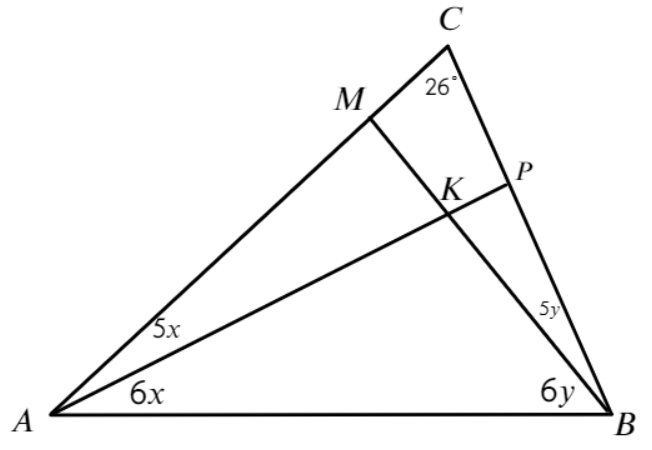
\includegraphics[scale=0.35]{g70.png}}
\end{figure}\\
Обозначим $\angle CAP=5x,\ \angle PAB=6x,\ \angle CBM=5y,\ \angle MBA=6y.$ Тогда из треугольника $ABC:\ 5x+6x+5y+6y+26^\circ=180^\circ,\ 11(x+y)=154^\circ,\ x+y=14^\circ.$ Теперь запишем сумму углов треугольника $AKB:\ 6x+6y+\angle AKB=180^\circ,\ \angle AKB=180^\circ-6(x+y)=180^\circ-6\cdot14^\circ=96^\circ.$\\
